\documentclass{article}

% required 
\usepackage[hyphens]{url} % this wraps my URL versus letting it spill across the page, a bad habit LaTeX has
\usepackage{Sweave}
\usepackage{graphicx}
\usepackage{natbib}
\usepackage{amsmath}
\usepackage{textcomp}%among other things, it allows degrees C to be added
\usepackage{float}
\usepackage[utf8]{inputenc} % allow funny letters in citations 
\usepackage[nottoc]{tocbibind} %should add Re fences to the table of contents?
\usepackage{amsmath} % making nice equations 
\usepackage{listings} % add in stan code
\usepackage{xcolor}
\usepackage{capt-of}%allows me to set a caption for code in appendix 
\usepackage[export]{adjustbox} % adding a box around a map
\usepackage{lineno}
\linenumbers
% recommended! Uncomment the below line and change the path for your computer!
% \SweaveOpts{prefix.string=/Users/Lizzie/Documents/git/teaching/demoSweave/Fig.s/demoFig, eps=FALSE} 
%put your Fig.s in one place! Also, note that here 'Fig.s' is the folder and 'demoFig' is what each 
% Fig. produced will be titled plus its number or label (e.g., demoFig-nqpbetter.pdf')
% make your captioning look better
\usepackage[small]{caption}

\usepackage{xr-hyper} %refer to Fig.s in another document
\usepackage{hyperref}

\setlength{\captionmargin}{30pt}
\setlength{\abovecaptionskip}{0pt}
\setlength{\belowcaptionskip}{10pt}

% optional: muck with spacing
\topmargin -1.5cm        
\oddsidemargin 0.5cm   
\evensidemargin 0.5cm  % same as odd side margin but for left-hand pages
\textwidth 15.59cm
\textheight 21.94cm 
% \renewcommand{\baselinestretch}{1.5} % 1.5 lines between lines
\parindent 0pt		  % sets leading space for paragraphs
% optional: cute, fancy headers
\usepackage{fancyhdr}
\pagestyle{fancy}
%\fancyhead[LO]{Frederik Baumgarten}
%\fancyhead[RO]{Research Proposal}
% more optionals! %

\graphicspath{ {/Users/frederik/github/PhaenoFlex_clean/analysis/output/} }% tell latex where to find figures 

\begin{document}
	\renewcommand{\bibname}{References}%names reference list 
	
	
	%	\title{
		%	} 
	
	
	\date{\today}
	
	\section*{Aim}
	As climate continues to warm, ecosystems are facing more extreme heat and drought waves. At the same time the potential growing season of temperate and boreal latitudes extends. To which degree plants and forests adapt and indeed prolong their photosynthetic activity in spring and autumn is currently under heavy debate. Not only may soil moisture resources limit plant activity and overall performance but also internal growth control mechanisms could limit further Carbon uptake from the atmosphere. Therefore, this experimental study aimed to provide evidence how longer climatic growing seasons translate into increased biomass production in relation to the negative impacts of drought and heat events. 
	
	\section*{Methods}
	\subsection*{Study species and study site}
	3 year-old saplings of 4 species, each representing a different family were selected to get a wide range of possible tree responses including coniferous evergreen and broad leaved deciduous species. All species selected occur naturally along the Pacific west coast of USA and Canada. The studied deciduous trees were Prunus virginiana L., Acer macrophyllum Pursh., Betula papyfera Marsh. and Quercus garryana Dougl.; evergreen trees were Pinus contorta Dougl., and Sequoia sempervirens (D. Don) Endl. \\
	
	The study was conducted at Totem Field located on the campus of the University of British Columbia (49.2572 N, -123.2503 E) in a typical oceanic climate. 
	
		\begin{figure}
		\centering
		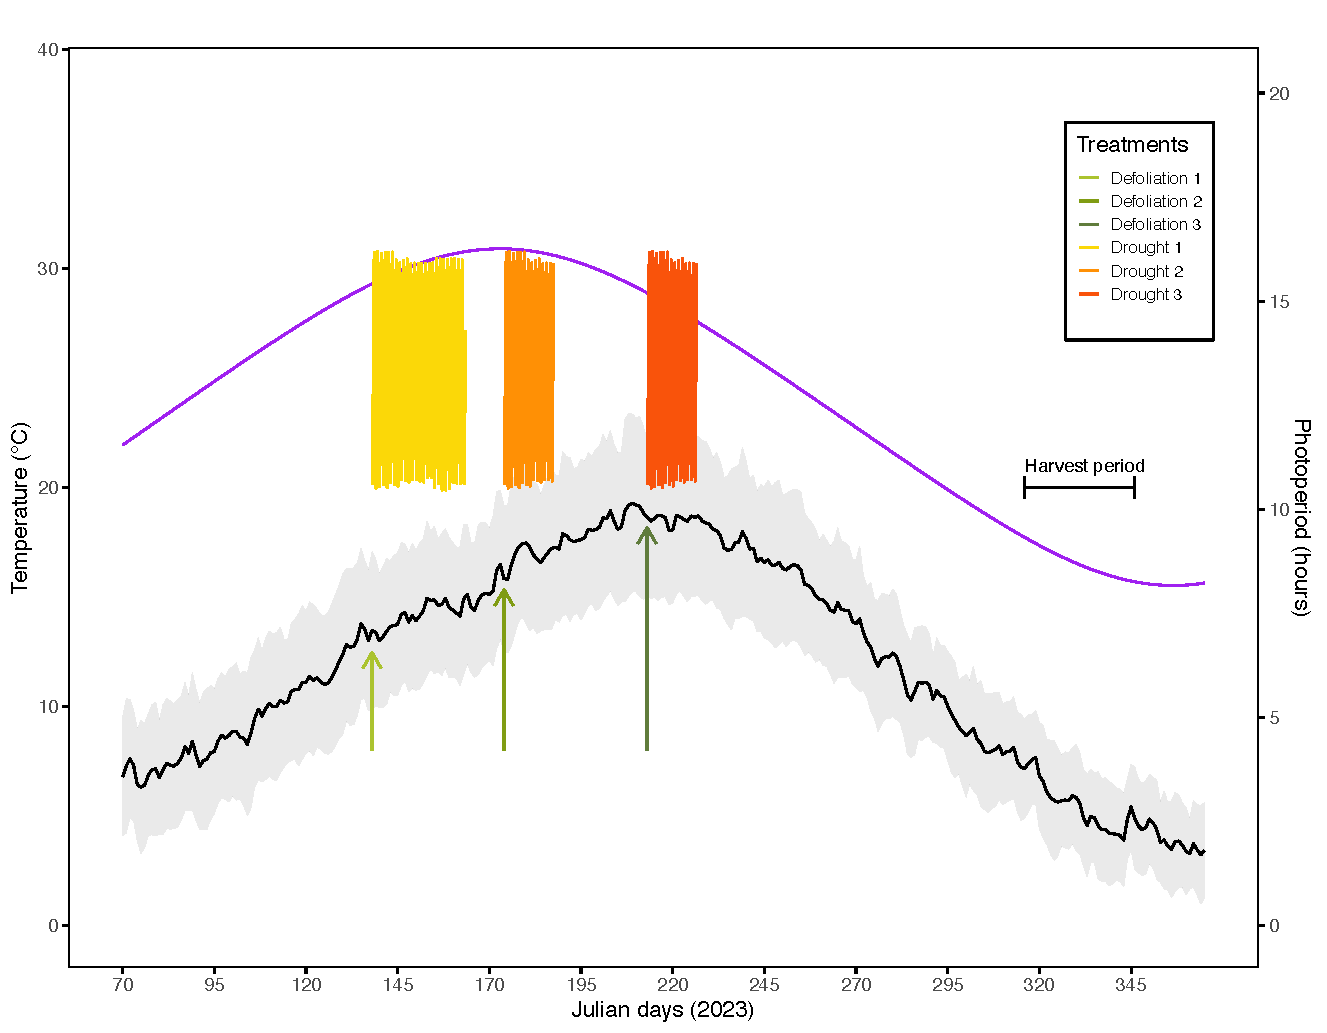
\includegraphics[width=0.9\textwidth]{design.pdf} 
		\caption{Effect size in g of biomass compared to control sapling when exposed to an extended growing season (GS\_extend), heat, defoliation or drought event. Colors represent the six study species. }
		\label{fig:fig_1xxx}
	\end{figure}
	
	\subsection*{Treatments}
	The whole study design is depicted in Fig. 1 for an overview. Plants arrived in full dormancy in April 2023 and were stored in cooling chambers at 4 °C to prolong dormancy. Of xx saplings per species 15 replicates were subjected to the following treatments: 1) growing season extension 
	
	
	\section*{Preliminary results}
	
	
	\begin{figure}
	\centering
	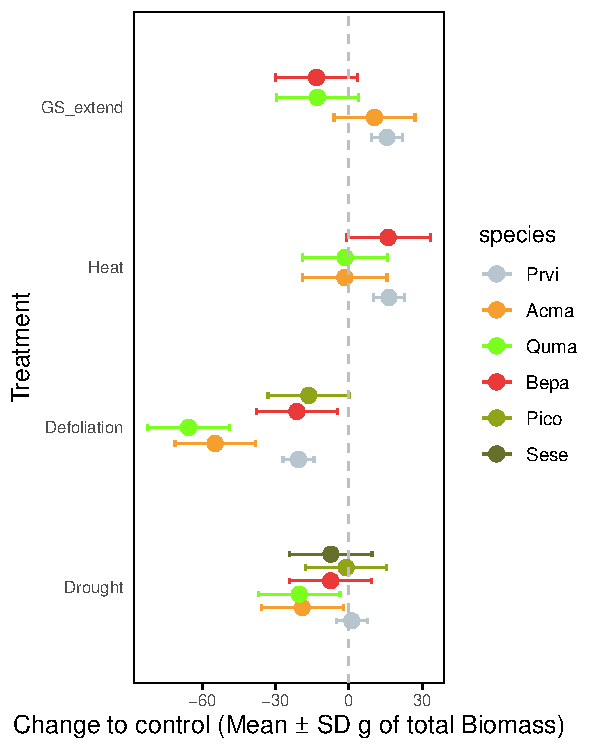
\includegraphics[width=0.9\textwidth]{posteriors/biomass_post_solst_treat_sub.pdf} 
	\caption{Effect size in g of biomass compared to control sapling when exposed to an extended growing season (GS\_extend), heat, defoliation or drought event. Colors represent the six study species. }
	\label{fig:fig_1xxx}
\end{figure}
	
	
			\begin{figure}
		\centering
		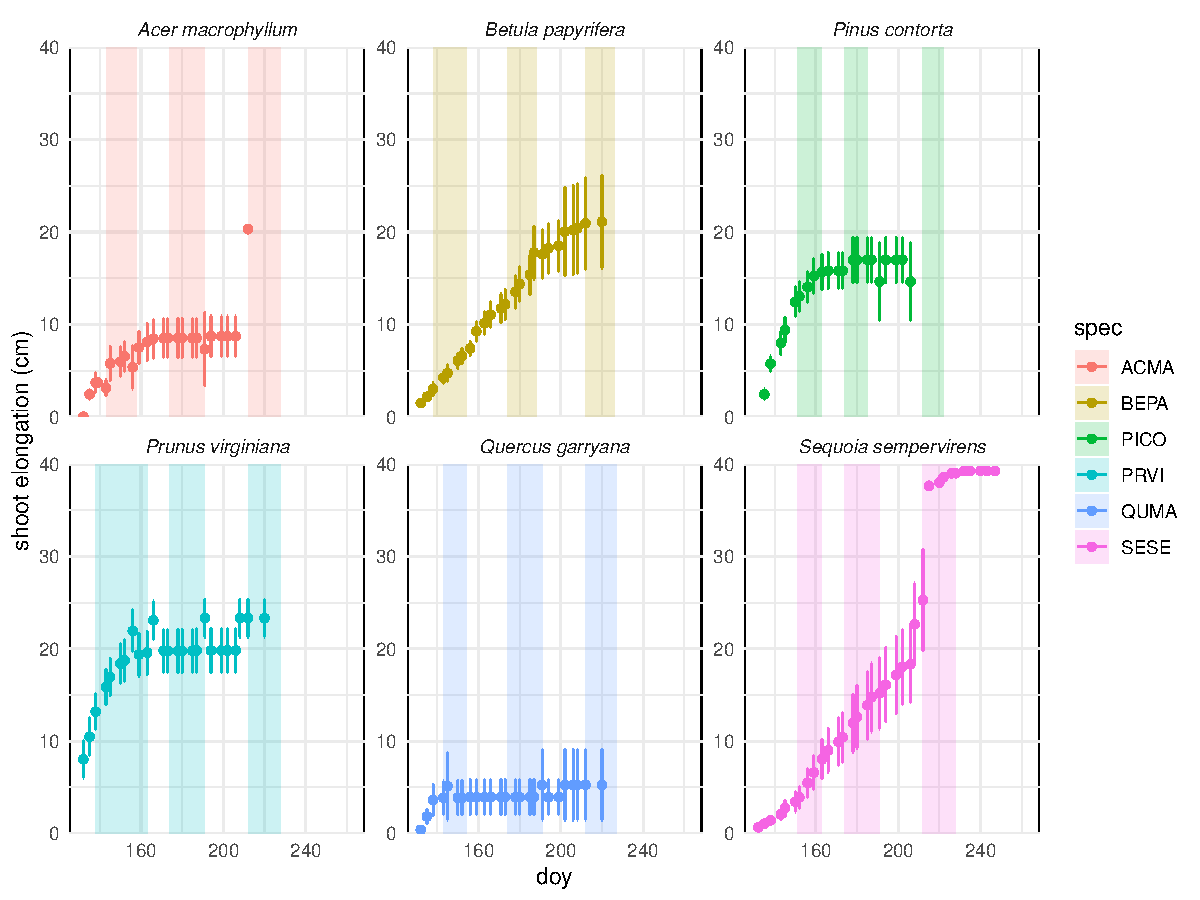
\includegraphics[width=0.9\textwidth]{shoot_elongation copy.pdf} 
		\caption{Shoot extension over the growing season 2023 for the six study species. Note the species-specific differences in absolute growth and in growth phenology with Quercus stopping first and Sequoia elongating until the very end of the season.}
		\label{fig:fig_1xxx}
	\end{figure}
	
	
				\begin{figure}
		\centering
		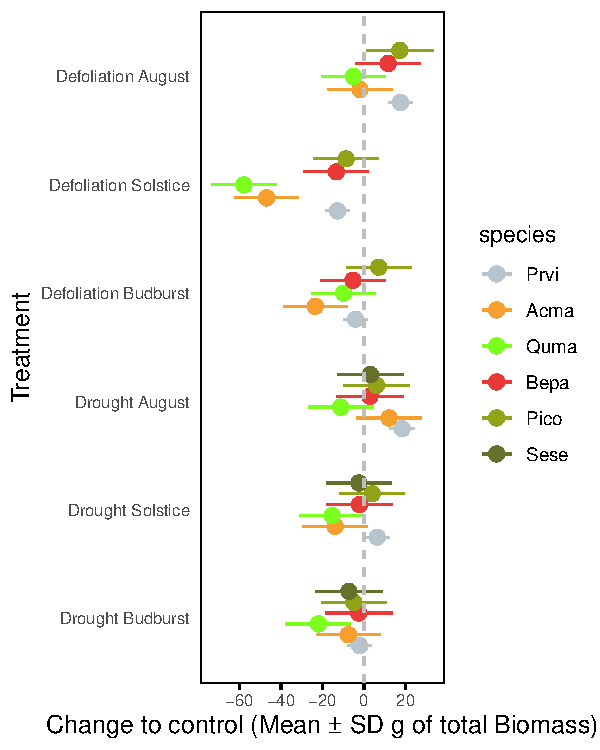
\includegraphics[width=0.9\textwidth]{posteriors/biomass_post_treat_sub.pdf} 
		\caption{Effect size in g of biomass compared to control sapling when exposed to defoliation or drought treatments on 3 occasions. Colors represent the six study species.}
		\label{fig:fig_1xxx}
	\end{figure}
	
	
	
	All treatments were conducted at Totem Field located on the campus of the University of British Columbia (49.2572, -123.2503) which has a moderate oceanic climate This climate leads to recurring droughts during the summer. Vancouver has been subjected to heat waves in the past years. For instance, the greater Vancouver area has been strucked with severe heat waves in 2009 and 2021 that lasted extended periods (Henderson et al., 2016; Henderson, McLean, Lee, Kosatsky, 2022). In addition of those very rare temperature, 2021 heat dome was characterised by near peak daylight hours and high night temperature (Henderson et al., 2022). In the past 20 years, the mean annual temperature on UBC campus was *** °C. and the annual precipitation is ***mm.
	\subsection*{Experimental Design}			The whole study design is depicted in Fig. 1 for an overview. Plants arrived in full dormancy in April 2023 and were stored in cooling chambers (Biochambers XXX) at 4 °C. to prolong dormancy until 1 May 2023. By releasing plants into a slightly progressed spring allowed to clearly define the climatic growing season (Körner und Hoch, 2023) without fluctuations around the temperature threshold of 5 °C where significant growth is known to occur (REF). 
	Still in dormancy all XX plants (xx per species) were re-potted using a medium for perennials consisting of 50% peat, 25% crushed pumice and 25% crushed bark (www.westcreekfarm.com) on 1, 2 and 3 May 2023. The low water-retention capacity of this potting medium allowed to accelerate and intensify the effects of the drought treatments. Soil volume was adjusted for each species, specifically doubled in volume compared to the previous container to minimize limitations later in the season (final pot volume: 4.5l for Sequoia and Pinus; 9l for Quercus and Betula; 18l for Acer, Prunus and Populus). 
	After potting, saplings received an equivalent of xx mg/ha of slow-release NPK fertilizer to meet natural conditions. Saplings were then arranged in 3 blocks, so that five replicates per treatment were in a different
	Three replicate blocks were established in which each had 5 replicates of all the treatments, for a total of 15 replicates per treatment. Two of those were in the greenhouse, and the third was on the north side of the greenhouse. A shelter was necessary to avoid damaging the dendrometers with rain water. Additionally, to limit heat accumulation at the top, a fan on the gable of the greenhouse was installed and the bottow plastic sides were opened to create air flow and consequently create similar temperature conditions for all three blocks, as showed by temperature sensors (HOBO, see supplement). These were installed in and outside of the greenhouse, on a pole at the following heights: 30 cm, 100 cm and 200cm. 
	\textit{Irrigation}:
	Moreover, we installed a drip irrigation system from Netafilm that dropped 120±6 ml of water withing 5 minutes, every 6 hours (i.e. 480ml/day) to permanently saturate soil moisture and avoid moisture differences between the different blocks. The irrigation controller was from Toro and the frame was built with schedule 40 PVC.
	
	\begin{table}[h!]
		\begin{center}
			\caption{Details of saplings origin }
			\label{tab:table1}
			\begin{tabular}{l|c|r} % 
				\textbf{Species} & \textbf{Nursery} & \textbf{Seed origin}\\
				%$\alpha$ & $\beta$ & $\gamma$ \\
				\hline
				Prunus virginiana L. & Peel's Nurseries Ltd. & BC Canada\\
				Acer macrophyllum Pursh. & Streamside Native Plants & BC Canada\\
				Betula papyfera Marsh. & Peel's Nurseries Ltd. &BC Canadac\\
				Quercus garryana ?.& Peel's Nurseries Ltd. & BC Canada\\
				Populus trichocarpa Torr. & Peel's Nurseries Ltd.& BC Canada\\
				Pinus contorta, Dougl. & Tree Time Services Inc & Alberta Canada\\
				Sequoia sempervirens(D. Don)&? & California\\
				
			\end{tabular}
		\end{center}
	\end{table}
	
	\subsection*{Drought treatments}
	//move here the general timings and explanations as this is the main treatment//
	
	Dendrometer installation //could you provide information on the software, location where they were build, etc.// 
	Once all the trees were in their respective blocks and drip irrigation installed, we set up the dendrometers on the control replicates and the first drought treatment replicates. 
	//reminder: tape //
	
	Swiss dendrometers
	//update this section//
	
	Climate chambers temperature and humidity
	We set the climate chambers to identical conditions for all drought treatments. The night temperature was set at 20 °C and the day temperature was set to 30 °C. These temperatures rose and fell at the same time every day, which corresponds to the time of sunrise and sunset at Vancouver’s summer solstice (i.e. 16h and 15min). The photoperiod was adjusted weekly, to the current ambient sunrise and sunset time. Hence. Four climate chambers from *** and one walk in chamber from *** were used and all of them are located in UBC’S Faculty of Forestry’s basement. For the first drought treatment dehumidifiers (Toshiba TDDP2213ES2) were set in the climate chambers at a set humidity of 35%, in order to avoid relative humidity differences that could affect the tree’s transpiration rate //should we add the date at which they were added?//. Indeed, if one growth chamber has a higher relative humidity than another, the plants in this one would reach the wilting point later than the others. 
	
	Dro 1 start decision:
	The first drought treatment started species-specific once leaf-out reached stage 4 (i.e. leaves fully unfolded). Specifically, the plants were moved to climate chambers () where they experienced 30 °C. during the day and 20 °C. during the night. While temperature cycles were constant across all four drought treatments to ensure comparability, the photoperiod followed ambient conditions, between treatments The trees were left to dry in the chambers for different periods depending on the species. For the first drought treatment, we removed the trees once one replicate from a species showed drought stress morphological symptoms. We assumed that at least one replicate reached their species’ wilting point. The removal decision was made on a species-specific basis and was arbitrary, as we observed distinct variations in the speed of symptom manifestation and their severity among individuals within the replicates of a single species. To avoid high mortality rate, we decided to remove all the replicates once one showed severe desiccation symptoms. The trees were then removed from the climate chambers, saturated with water, and reintroduced in the field, where they were reconnected to the irrigation system. Dendrometers were kept on these replicates for a minimum period of two weeks to monitor radial growth following this drought treatment. After this, the dendrometers were placed on the second drought treatment replicates for 5 to 7 days which allowed us to monitor radial growth prior to their shift in the climate chambers.
	
	Dro 2, 3, 4 start decision
	The replicates selected for the following drought treatments were all moved at the same time. The decision of removal for the second drought treatment was slightly different. Since we had access to the rate of water loss and the VWC at which the replicates from the first drought treatment reached their wilting point, we included these factors in the decision process. // Should we mention the decision steps we discussed. Would a simple figure be a good idea for this // Once all the replicates were removed from the climate chambers, they stayed in the field for two weeks for radial monitoring, then the dendrometers were set for the following drought treatment //(idem for dro1, 2, 3, 4, how could we avoid repetition?//
	
	
	\subsection*{Defoliation treatments}
	Two defoliation treatments were applied at the same time during the summer, one that started on May 16th, and the second, on June 23rd. Those treatments were designed to mimic a net loss of leaf area induced by either browsing, spring frost or drought. 
	
	Timing:
	•	We conducted the first defoliation treatment once the leaves from most of the replicates of one species have reached the fourth phenological stage. This stage was reached at different times, depending on the species, therefore, the start of this treatment was species-specific. 
	•	The second defoliation treatment was conducted after the theoretical peak growth period that happens around summer solstice. At that time, all species have reached the fourth phenological stage. 
	
	Defoliation:
	Deciduous trees 
	Using pruning snips (Fiskars Garden), we cut all the leaves mid petiole that were at phenological stage 4. We selected this technique which was in several studies (Miller Tworkoski, 2010; Nzima, Martin, Nishijima, 1999).Younger stages were left intact to not accidentally damage the terminal meristem. In the following two weeks we continuously cut all newly emerging leaves reaching stage 4 to suspend all assimilate supply.
	
	Evergreen (Pinus)
	All one-year-old and older mature needles were removed by hand by tearing them delicately in the direction of the apex to not hurt the bark as mentioned in (O’Neil, 2011). The current year needles were preserved in the first defoliation treatment since they were less than 1cm in length and still developing. In the second treatment we additionally defoliated c. ¾ of the current-year needles which were still not fully elongated but presumably contributed already most to the total photosynthetic assimilation.
	//I think we should mention here the weight of the leaves we removed. Perhaps we make a table out of that. //
	
	Drying:
	All the leaves collected were gathered in brown paper bags, where all the replicates from the same species were put together to dry. The leaves were dried for 48 hours at 70°C in a drying oven (VWR 1645D). Dry matter biomass was measured with scale (Scout Pro) to an accuracy of two decimal places (0.00 grams).
	
	\subsection*{Soil moisture measurements}
	Everyday, at the same time, the volumetric water content (VWC) was measured using a soil moisture meter (Fieldscout TDR 150). The rod length was changed depending on the pot depth that varied for different species (i.e. …). One was 12.2 cm and the other was 20.32 cm. In addition, and for a more integrated indicator of soil water loss especially near the wilting point, whole pots were weighted using a scale (REF) to an accuracy of 1 gram. To avoid noise in the radial monitoring data, replicates equipped with magnetic dendrometers were only weighted at the start and end of the drought treatments. Since VWC and weight loss yielded a strong correlation (Fig SX) whole VWC curves were calculated also for these replicates.
	
	
	
	
	
	\begin{figure}
		\centering
		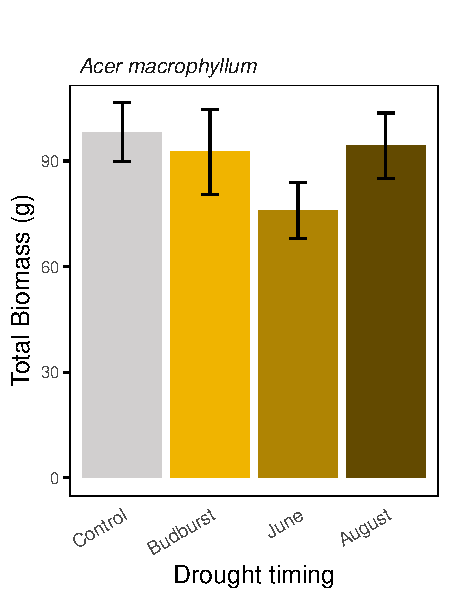
\includegraphics[width=0.9\textwidth]{biomass_tot_Acma.pdf} 
		\caption{xxxxxxxxxxx}
		\label{fig:fig_1xxx}
	\end{figure}
	
	
	
	\section*{stuff I did't find place yet}
	
	
	\newpage
	
	
	\bibliography{Art_simulation}
	\bibliographystyle{ecolett}
	
	
	
	
	
	
\end{document}
